\documentclass[a4paper]{article}
\usepackage{fontspec}\defaultfontfeatures{Ligatures=TeX}
%-----------------------------------------------------------------------------%
\usepackage{tufte-settings}
%-----------------------------------------------------------------------------%
%%% Title %%%
\title{Tufte Document Example}
\author{Jesse C.\ Chen}
\date{\today}
%-----------------------------------------------------------------------------%

\begin{document}

\maketitle

\noindent
Lorem ipsum dolor sit amet, consectetuer adipiscing elit. Aenean commodo ligula
eget dolor. Aenean massa. Cum sociis natoque penatibus et magnis dis parturient
montes, nascetur ridiculus mus. Donec quam felis, ultricies nec, pellentesque.

\begin{marginfigure}
	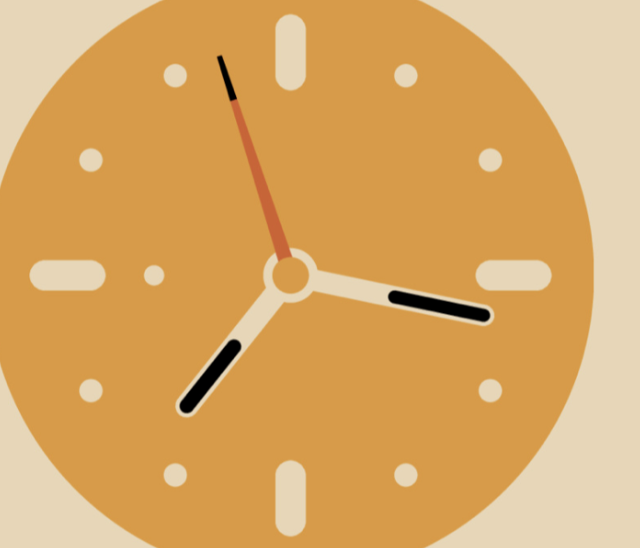
\includegraphics[width=\marginparwidth]{test-1.png}
	\caption{A cube represented as the 6 square faces that bound it}
	\label{fig:brep}
\end{marginfigure}

Nulla consequat massa quis enim. Donec pede justo,
\footnote{\label{foot:first}%
	This is a footnote.
}
fringilla vel, aliquet nec, vulputate eget, arcu. In enim justo, rhoncus ut,
imperdiet a, venenatis vitae, justo. Nullam dictum felis eu pede mollis
pretium. Integer tincidunt. Cras dapibus. Vivamus elementum semper nisi. Aenean
vulputate eleifend tellus. Aenean leo ligula, porttitor eu, consequat vitae,
eleifend ac, enim. Aliquam lorem ante, dapibus in, viverra quis, feugiat a,
tellus. Phasellus viverra nulla ut metus varius laoreet. Quisque rutrum.

\begin{figure*}[t!]
	\centering
	
\includegraphics[width=\linewidth]{test-2.png}
	\caption{Full-width Picture.}
	\label{fig:full-width}
\end{figure*}

Lorem ipsum dolor sit amet, consectetuer adipiscing elit. Aenean commodo ligula
eget dolor. Aenean massa. Cum sociis natoque penatibus et magnis dis parturient
montes, nascetur ridiculus mus. Donec quam felis, ultricies nec, pellentesque
eu, pretium quis, sem. Nulla consequat massa quis enim. Donec pede justo,
fringilla vel, aliquet nec, vulputate eget, arcu. In enim justo, rhoncus ut,
imperdiet a, venenatis vitae, justo. Nullam dictum felis eu pede mollis
pretium. Integer tincidunt. Cras dapibus. Vivamus elementum semper nisi. Aenean
vulputate eleifend tellus. Aenean leo ligula, porttitor eu, consequat vitae,
eleifend ac, enim. Aliquam lorem ante, dapibus in, viverra quis, feugiat a,
tellus. Phasellus viverra nulla ut metus varius laoreet. Quisque rutrum.

\begin{figure}[h]
	\sidecaption[][]{Textwidth Figure.\label{fig:textwidth}}
	
\includegraphics[width=\linewidth]{test-2.png}
\end{figure}

Lorem ipsum dolor sit amet, consectetuer adipiscing elit. Aenean commodo ligula
eget dolor. Aenean massa. Cum sociis natoque penatibus et magnis dis parturient
montes, nascetur ridiculus mus. Donec quam felis, ultricies nec, pellentesque
eu, pretium quis, sem. Nulla consequat massa quis enim. Donec pede justo,
\footnote{\label{foot:second}%
	Lorem ipsum dolor sit amet, consectetuer adipiscing elit. Aenean commodo ligula
	eget dolor. Aenean massa. Cum sociis natoque penatibus et magnis dis parturient
	montes, nascetur ridiculus mus
	\autoref{fig:textwidth}.
}
fringilla vel, aliquet nec, vulputate eget, arcu. In enim justo, rhoncus ut,
imperdiet a, venenatis vitae, justo. Nullam dictum felis eu pede mollis
pretium. Integer tincidunt. Cras dapibus. Vivamus elementum semper nisi. Aenean
Please refer to \autoref{foot:first}.

\end{document}
